\chapter{Especificación de casos de uso}
\label{chap:casos_uso}

\section{CU1. Registro}
\label{sec:cu:registro}

\begin{table}[H]
    \centering
    \begin{tabular}{|p{0.25\textwidth} p{0.75\textwidth}|}
    \hline
    \multicolumn{2}{|l|}{\textbf{Caso de Uso 1. Registro}} \\ \hline \hline
    Requisitos          & \labelcref{req:registro} \\ \hline
    Precondiciones      & La cuenta de Google del usuario no debe estar registrada \\ \hline
    Actores             & Usuarios no registrados \\ \hline
    Descripción         & Un usuario nuevo se creará un perfil del sistema e iniciará sesión \\ \hline
    Secuencia normal    & El usuario abrirá la aplicación por primera vez \\
                        & Seleccionará el botón de \emph{Iniciar Sesión} \\
                        & Seleccionará su cuenta de Google \\
                        & Introducirá un nombre para identificarse \\
                        & Elegirá el rol que desee \\
                        & Incluirá su información de contacto adicional \\
                        & Confirmará los datos introducidos \\
                        & El usuario será dirigido a la pantalla principal con un nuevo perfil \\ \hline
    Postcondiciones     & -  \\ \hline
    Excepciones         & Cuenta de Google ya usada: Se iniciará sesión normalmente  \\ \hline
    \end{tabular}
    \caption{Especificación del CU1. Registro}
    \label{cu:registro}
\end{table}

\section{CU2. Iniciar sesión}
\label{sec:cu:iniciar_sesion}

\begin{longtable}{|p{0.25\textwidth} p{0.75\textwidth}|}
    \hline
    \multicolumn{2}{|l|}{\textbf{Caso de Uso 2. Iniciar sesión}} \\ \hline \hline
    Requisitos          & \labelcref{req:inicio_sesion} \\ \hline
    Precondiciones      & El usuario debe disponer de un perfil en el sistema \\ \hline
    Actores             & Pacientes y Cuidadores \\ \hline
    Descripción         & El usuario iniciará sesión con su perfil en el sistema \\ \hline
    Secuencia normal    & El usuario abrirá la aplicación \\
                        & Seleccionará el botón de \emph{Iniciar Sesión} \\
                        & Seleccionará su cuenta de Google \\
                        & El usuario será dirigido a la pantalla principal con su perfil \\ \hline
    Postcondiciones     & - \\ \hline
    Excepciones         & - \\ \hline
    \caption{Especificación del CU2. Iniciar sesión}
    \label{cu:iniciar_sesion}
\end{longtable}

\begin{figure}[H]
    \centering
    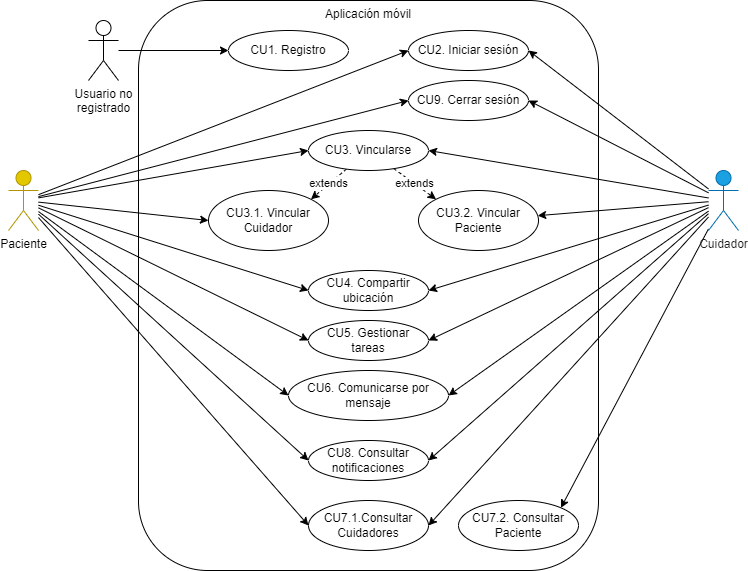
\includegraphics[width=0.85\textwidth]{images/Analisis/CasosUsoGeneral.drawio.png}
    \caption{Diagrama de casos de uso generales}
    \label{fig:casos_uso_general}
\end{figure}

\section{CU3. Vincularse con otro usuario}
\label{sec:cu:vinculacion}

\begin{longtable}{|p{0.25\textwidth} p{0.75\textwidth}|}
    \hline
    \multicolumn{2}{|l|}{\textbf{Caso de Uso 3.1. Vincular un Cuidador}} \\ \hline \hline
    Requisitos          & \labelcref{req:vinculo_paciente} \\ \hline
    Precondiciones      & El usuario debe haber iniciado sesión \\
                        & El Cuidador a vincular debe estar cerca y preparado \\ \hline
    Actores             & Pacientes \\ \hline
    Descripción         & El usuario generará un código para vincularse con un Cuidador \\ \hline
    Secuencia normal    & El usuario seleccionará la función \emph{Forjar vínculo} \\
                        & Un código QR se mostrará en su pantalla \\
                        & El Cuidador lo escaneará \\
                        & Se creará el vínculo entre los usuarios y se notificará a los usuarios asociados \\ \hline
    Postcondiciones     & - \\ \hline
    Excepciones         & El Paciente no puede vincular más Cuidadores: No se forjará el vínculo \\ \hline
    \caption{Especificación del CU3.1. Vincular un Cuidador}
    \label{cu:vincular_cuidador}
\end{longtable}

\begin{longtable}{|p{0.25\textwidth} p{0.75\textwidth}|}
    \hline
    \multicolumn{2}{|l|}{\textbf{Caso de Uso 3.2. Vincular un Paciente}} \\ \hline \hline
    Requisitos          & \labelcref{req:vinculo_cuidador} \\ \hline
    Precondiciones      & El usuario debe haber iniciado sesión \\
                        & El usuario no debe estar ya vinculado \\ 
                        & El Paciente a vincular debe estar cerca y con su código preparado \\ \hline
    Actores             & Cuidadores \\ \hline
    Descripción         & El usuario leerá un código para vincularse con un Paciente \\ \hline
    Secuencia normal    & El usuario seleccionará la función \emph{Forjar vínculo} \\
                        & La aplicación solicitará permisos para utilizar la cámara \\
                        & El usuario aceptará la petición \\
                        & El usuario escaneará el código del Paciente \\
                        & Se creará el vínculo entre los usuarios y se notificará a los asociados \\ \hline
    Postcondiciones     & - \\ \hline
    Excepciones         & No se dan los permisos: La función no se iniciará \\
                        & El Paciente no puede vincular más Cuidadores: No se forjará el vínculo \\ \hline
    \caption{Especificación del CU3.2. Vincular un Paciente}
    \label{cu:vincular_paciente}
\end{longtable}

\begin{longtable}{|p{0.25\textwidth} p{0.75\textwidth}|}
    \hline
    \multicolumn{2}{|l|}{\textbf{Caso de Uso 3.3. Desvincularse}} \\ \hline \hline
    Requisitos          & \labelcref{req:borrar_vinculo} \\ \hline
    Precondiciones      & El usuario debe haber iniciado sesión \\
                        & El usuario debe estar vinculado \\ \hline
    Actores             & Pacientes y Cuidadores \\ \hline
    Descripción         & El usuario eliminará uno de sus vínculos \\ \hline
    Secuencia normal    & El usuario seleccionará la función \emph{Eliminar vínculo} \\
                        & El usuario seleccionará el vínculo a eliminar \\
                        & La aplicación le pedirá confirmación \\
                        & Se eliminará el vínculo entre los usuarios y se notificará a los usuarios asociados \\ \hline
    Postcondiciones     & - \\ \hline
    Excepciones         & - \\ \hline
    \caption{Especificación del CU3.3. Desvincularse}
    \label{cu:desvincular}
\end{longtable}

\section{CU4. Compartir ubicación}
\label{sec:cu:ubicacion}

\begin{longtable}{|p{0.25\textwidth} p{0.75\textwidth}|}
    \hline
    \multicolumn{2}{|l|}{\textbf{Caso de Uso 4.1. Compartir ubicación del usuario}} \\ \hline \hline
    Requisitos          & \labelcref{req:compartir_ubicacion} \\ \hline
    Precondiciones      & El usuario debe haber iniciado sesión \\
                        & El usuario debe estar vinculado \\ \hline
    Actores             & Pacientes y Cuidadores \\ \hline
    Descripción         & El usuario enviará su ubicación actual a los usuarios asociados \\ \hline
    Secuencia normal    & El usuario seleccionará la función \emph{Compartir ubicación} \\
                        & La aplicación solicitará permisos para acceder a la ubicación \\
                        & El usuario aceptará la petición \\
                        & Se desplegará un mapa mostrando la ubicación del usuario \\
                        & Empezará a compartirse la ubicación del usuario y se notificará a los asociados \\ \hline
    Postcondiciones     & - \\ \hline
    Excepciones         & No se dan los permisos: La función no se iniciará \\ \hline
    \caption{Especificación del CU4.1. Compartir ubicación del usuario}
    \label{cu:compartir_ubicacion}
\end{longtable}

\begin{longtable}{|p{0.25\textwidth} p{0.75\textwidth}|}
    \hline
    \multicolumn{2}{|l|}{\textbf{Caso de Uso 4.2. Ver ubicaciones de usuarios asociados}} \\ \hline \hline
    Requisitos          & \labelcref{req:ver_ubicaciones} \\ \hline
    Precondiciones      & El usuario debe haber iniciado sesión \\
                        & El usuario debe estar vinculado \\
                        & Los usuarios asociados deben estar compartiendo su ubicación  \\ \hline
    Actores             & Pacientes y Cuidadores \\ \hline
    Descripción         & La aplicación mostrará al usuario la ubicación de sus usuarios asociados \\ \hline
    Secuencia normal    & El usuario seleccionará la función \emph{Compartir ubicación} \\
                        & El usuario empezará a compartir su ubicación (véase \ref{cu:compartir_ubicacion}) \\
                        & Se desplegará un mapa mostrando la ubicación de los usuarios conectados \\ \hline
    Postcondiciones     & Si el usuario deja de compartir su ubicación no podrá ver las del resto \\ \hline
    Excepciones         & - \\ \hline
    \caption{Especificación del CU4.2. Ver ubicaciones de usuarios asociados}
    \label{cu:ver_ubicaciones}
\end{longtable}

\section{CU5. Gestionar tareas}
\label{sec:cu:tareas}

\begin{longtable}{|p{0.25\textwidth} p{0.75\textwidth}|}
    \hline
    \multicolumn{2}{|l|}{\textbf{Caso de Uso 5.1. Listar tareas}} \\ \hline \hline
    Requisitos          & \labelcref{req:listar_tarea} \\ \hline
    Precondiciones      & El usuario debe haber iniciado sesión \\
                        & Si es Cuidador debe estar vinculado \\ \hline
    Actores             & Pacientes y Cuidadores \\ \hline
    Descripción         & El usuario consultará la lista de tareas relevantes que tiene asociadas \\ \hline
    Secuencia normal    & El usuario seleccionará la pantalla \emph{Tareas} o \emph{Feed} \\
                        & La aplicación recuperarás las tareas relevantes asociadas al usuario \\
                        & Las tareas recuperadas se mostrarán en la pantalla \\ \hline
    Postcondiciones     & - \\ \hline
    Excepciones         & - \\ \hline
    \caption{Especificación del CU5.1. Listar tareas}
    \label{cu:listar_tareas}
\end{longtable}

\begin{longtable}{|p{0.25\textwidth} p{0.75\textwidth}|}
    \hline
    \multicolumn{2}{|l|}{\textbf{Caso de Uso 5.2. Crear tarea}} \\ \hline \hline
    Requisitos          & \labelcref{req:crear_tarea} \\ \hline
    Precondiciones      & El usuario debe haber iniciado sesión \\
                        & Si es Cuidador debe estar vinculado \\ \hline
    Actores             & Pacientes y Cuidadores \\ \hline
    Descripción         & El usuario creará una tarea que se compartirá con los demás usuarios asociados \\ \hline
    Secuencia normal    & El usuario seleccionará la pantalla \emph{Tareas} o \emph{Feed} \\
                        & El usuario seleccionará la función \emph{Crear tarea} \\
                        & El usuario rellenará los campos obligatorios \\
                        & El usuario rellenará los campos opcionales que desee \\
                        & El usuario confirmará la creación de la tarea \\
                        & El sistema creará la tarea y la notificará a los demás usuarios asociados \\ \hline
    Postcondiciones     & - \\ \hline
    Excepciones         & - \\ \hline
    \caption{Especificación del CU5.2. Crear tarea}
    \label{cu:crear_tarea}
\end{longtable}

\begin{longtable}{|p{0.25\textwidth} p{0.75\textwidth}|}
    \hline
    \multicolumn{2}{|l|}{\textbf{Caso de Uso 5.3. Marcar tarea como hecha}} \\ \hline \hline
    Requisitos          & \labelcref{req:marcar_tarea_hecha} \\ \hline
    Precondiciones      & El usuario debe haber iniciado sesión \\
                        & Si es Cuidador debe estar vinculado \\ 
                        & Debe existir alguna tarea no hecha asociada al usuario \\ \hline
    Actores             & Pacientes y Cuidadores \\ \hline
    Descripción         & El usuario marcará una tarea asociada como hecha \\ \hline
    Secuencia normal    & El usuario listará sus tareas, véase CU5.1 (\ref{cu:listar_tareas}) \\
                        & El usuario seleccionará la tarea no hecha que desee \\
                        & El usuario marcará la opción de marcarla hecha \\
                        & La aplicación pedirá confirmación al usuario \\
                        & El usuario confirmará la acción \\
                        & Se modificará la tarea y se notificará a los usuarios asociados \\ \hline
    Postcondiciones     & - \\ \hline
    Excepciones         & - \\ \hline
    \caption{Especificación del CU5.3. Marcar tarea como hecha}
    \label{cu:marcar_tarea}
\end{longtable}

\begin{longtable}{|p{0.25\textwidth} p{0.75\textwidth}|}
    \hline
    \multicolumn{2}{|l|}{\textbf{Caso de Uso 5.4. Desmarcar tarea hecha}} \\ \hline \hline
    Requisitos          & \labelcref{req:marcar_tarea_no_hecha} \\ \hline
    Precondiciones      & El usuario debe haber iniciado sesión \\
                        & Si es Cuidador debe estar vinculado \\ 
                        & Debe existir alguna tarea hecha asociada al usuario \\ \hline
    Actores             & Pacientes y Cuidadores \\ \hline
    Descripción         & El usuario desmarcará una tarea marcada como hecha \\ \hline
    Secuencia normal    & El usuario listará sus tareas, véase CU5.1 (\ref{cu:listar_tareas}) \\
                        & El usuario seleccionará la tarea hecha que desee \\
                        & El usuario marcará la opción de marcarla como no hecha \\
                        & La aplicación pedirá confirmación al usuario \\
                        & El usuario confirmará la acción \\
                        & Se modificará la tarea y se notificará a los usuarios asociados \\ \hline
    Postcondiciones     & - \\ \hline
    Excepciones         & - \\ \hline
    \caption{Especificación del CU5.4. Desmarcar tarea hecha}
    \label{cu:desmarcar_tarea}
\end{longtable}

\begin{longtable}{|p{0.25\textwidth} p{0.75\textwidth}|}
    \hline
    \multicolumn{2}{|l|}{\textbf{Caso de Uso 5.5. Eliminar tarea}} \\ \hline \hline
    Requisitos          & \labelcref{req:eliminar_tarea} \\ \hline
    Precondiciones      & El usuario debe haber iniciado sesión \\
                        & Si es Cuidador debe estar vinculado \\ 
                        & Debe existir alguna tarea asociada al usuario \\ \hline
    Actores             & Pacientes y Cuidadores \\ \hline
    Descripción         & El usuario eliminará una tarea asociada \\ \hline
    Secuencia normal    & El usuario listará sus tareas, véase CU5.1 (\ref{cu:listar_tareas}) \\
                        & El usuario seleccionará la tarea que desee eliminar \\
                        & El usuario elegirá la opción de \emph{Eliminar} la tarea \\
                        & La aplicación pedirá confirmación al usuario \\
                        & El usuario confirmará la acción \\
                        & Se eliminará la tarea y se notificará a los asociados \\ \hline
    Postcondiciones     & - \\ \hline
    Excepciones         & El usuario no es el Paciente o el creador de la tarea: Se le comunicará que es una acción que no puede realizar y no se llevará a cabo \\ \hline
    \caption{Especificación del CU5.5. Eliminar tarea}
    \label{cu:eliminar_tarea}
\end{longtable}

\section{CU6. Comunicarse por mensaje instantáneo}
\label{sec:cu:mensajes}

\begin{longtable}{|p{0.25\textwidth} p{0.75\textwidth}|}
    \hline
    \multicolumn{2}{|l|}{\textbf{Caso de Uso 6.1. Ver mensajes}} \\ \hline \hline
    Requisitos          & \labelcref{req:listar_mensaje} \\ \hline
    Precondiciones      & El usuario debe haber iniciado sesión \\
                        & El usuario debe estar vinculado \\ \hline
    Actores             & Pacientes y Cuidadores \\ \hline
    Descripción         & El usuario verá sus mensajes y tareas asociadas \\ \hline
    Secuencia normal    & El usuario abrirá la pantalla \emph{Feed} \\
                        & La aplicación mostrará los mensajes y tareas asociados al usuario más recientes \\ 
                        & La aplicación mostrará los nuevos mensajes que vayan enviado los usuarios asociados \\ \hline
    Postcondiciones     & - \\ \hline
    Excepciones         & - \\ \hline
    \caption{Especificación del CU6.1. Ver mensajes}
    \label{cu:ver_mensajes}
\end{longtable}

\begin{longtable}{|p{0.25\textwidth} p{0.75\textwidth}|}
    \hline
    \multicolumn{2}{|l|}{\textbf{Caso de Uso 6.2. Enviar mensajes}} \\ \hline \hline
    Requisitos          & \labelcref{req:envio_mensaje} \\ \hline
    Precondiciones      & El usuario debe haber iniciado sesión \\
                        & El usuario debe estar vinculado \\ \hline
    Actores             & Pacientes y Cuidadores \\ \hline
    Descripción         & El usuario verá sus mensajes asociados \\ \hline
    Secuencia normal    & El usuario abrirá la pantalla \emph{Feed} \\
                        & El usuario redactará el mensaje que quiera enviar \\
                        & El usuario pulsará el botón de \emph{Enviar mensaje} \\
                        & El mensaje se listará en la pantalla del usuario \\
                        & El mensaje se enviará al resto de usuarios asociados \\ \hline
    Postcondiciones     & - \\ \hline
    Excepciones         & - \\ \hline
    \caption{Especificación del CU6.2. Enviar mensajes}
    \label{cu:enviar_mensajes}
\end{longtable}

\section{CU7. Consultar información de asociados}

\begin{longtable}{|p{0.25\textwidth} p{0.75\textwidth}|}
    \hline
    \multicolumn{2}{|l|}{\textbf{Caso de Uso 7.1. Consultar Cuidadores asociados}} \\ \hline \hline
    Requisitos          & \labelcref{req:consultar_info_cuidador} \\ \hline
    Precondiciones      & El usuario debe haber iniciado sesión \\
                        & El usuario debe estar vinculado \\ \hline
    Actores             & Pacientes y Cuidadores \\ \hline
    Descripción         & El usuario listará sus Cuidadores asociados y la información de estos \\ \hline
    Secuencia normal    & El usuario abrirá la pantalla \emph{Vínculos} \\
                        & La aplicación obtendrá el listado de los Cuidadores asociados al usuario \\
                        & Los cuidadores asociados se mostrarán en pantalla \\
                        & El usuario desplegará la información del Cuidador que desee para ver su información de contacto completa \\ \hline
    Postcondiciones     & - \\ \hline
    Excepciones         & - \\ \hline
    \caption{Especificación del CU7.1. Consultar Cuidadores asociados}
    \label{cu:consultar_cuidador}
\end{longtable}

\begin{longtable}{|p{0.25\textwidth} p{0.75\textwidth}|}
    \hline
    \multicolumn{2}{|l|}{\textbf{Caso de Uso 7.2. Consultar Paciente asociado}} \\ \hline \hline
    Requisitos          & \labelcref{req:consultar_info_paciente} \\ \hline
    Precondiciones      & El usuario debe haber iniciado sesión \\
                        & El usuario debe estar vinculado \\ \hline
    Actores             & Cuidadores \\ \hline
    Descripción         & El usuario consultará la información de su paciente asociado \\ \hline
    Secuencia normal    & El usuario abrirá la aplicación \\
                        & La aplicación recuperará la información del Paciente \\
                        & Se mostrará en la pantalla principal la información del Paciente \\
                        & El usuario desplegará la información del Paciente para ver su información de contacto completa \\ \hline
    Postcondiciones     & - \\ \hline
    Excepciones         & - \\ \hline
    \caption{Especificación del CU7.2. Consultar Paciente asociado}
    \label{cu:consultar_paciente}
\end{longtable}

\section{CU8. Consultar notificaciones}

\begin{longtable}{|p{0.25\textwidth} p{0.75\textwidth}|}
    \hline
    \multicolumn{2}{|l|}{\textbf{Caso de Uso 8.1 Consultar notificaciones no leídas}} \\ \hline \hline
    Requisitos          & \labelcref{req:consultar_notificaciones} \\ \hline
    Precondiciones      & El usuario debe haber iniciado sesión \\
                        & El usuario debe estar vinculado \\ \hline
    Actores             & Pacientes y Cuidadores \\ \hline
    Descripción         & El usuario consultará las notificaciones no leídas \\ \hline
    Secuencia normal    & El usuario abrirá la pantalla \emph{Notificaciones} \\
                        & La aplicación recuperará las notificaciones no leídas del usuario \\
                        & Las notificaciones recuperadas se mostrarán en la pantalla agrupadas \\ \hline
    Postcondiciones     & - \\ \hline
    Excepciones         & - \\ \hline
    \caption{Especificación del CU8.1 Consultar notificaciones no leídas}
    \label{cu:consultar_notificaciones}
\end{longtable}

\begin{figure}[H]
\begin{longtable}{|p{0.25\textwidth} p{0.75\textwidth}|}
    \hline
    \multicolumn{2}{|l|}{\textbf{Caso de Uso 8.2 Marcar notificaciones como leídas}} \\ \hline \hline
    Requisitos          & \labelcref{req:leer_notificaciones} \\ \hline
    Precondiciones      & El usuario debe haber iniciado sesión \\
                        & El usuario debe estar vinculado \\
                        & El usuario debe tener notificaciones pendientes no leídas \\ \hline
    Actores             & Pacientes y Cuidadores \\ \hline
    Descripción         & El usuario marcará uno o todas sus notificaciones pendientes como leídas \\ \hline
    Secuencia normal    & El usuario listará sus aplicaciones, véase CU8.1 (\ref{cu:consultar_notificaciones}) \\
                        & El usuario usará el botón \emph{Marcar como leída} de una notificación o \emph{Marcar todas como leídas} \\
                        & La notificación se marcará como leídas \\ \hline
    Postcondiciones     & - \\ \hline
    Excepciones         & - \\ \hline
    \caption{Especificación del CU8.2 Marcar notificaciones como leídas}
    \label{cu:marcar_notificaciones}
\end{longtable}
\end{figure}

\section{CU9. Cerrar sesión}

\begin{longtable}{|p{0.25\textwidth} p{0.75\textwidth}|}
    \hline
    \multicolumn{2}{|l|}{\textbf{Caso de Uso 9. Cerrar sesión}} \\ \hline \hline
    Requisitos          & \labelcref{req:cierre_sesion} \\ \hline
    Precondiciones      & El usuario debe haber iniciado sesión \\ \hline
    Actores             & Pacientes y Cuidadores \\ \hline
    Descripción         & El usuario seleccionará la función \emph{Cerrar sesión} \\ \hline
    Secuencia normal    & Se cerrará la sesión y se devolverá al usuario a la pantalla de \emph{Iniciar sesión} \\ \hline
    Postcondiciones     & - \\ \hline
    Excepciones         & - \\ \hline
    \caption{Especificación del CU9. Cerrar sesión}
    \label{cu:cerrar_sesion}
\end{longtable}